\documentclass{article}
%\usepackage{fullpage}
\usepackage{fancyhdr}
\usepackage[english,francais]{babel}
\usepackage[T1]{fontenc}
\usepackage[utf8]{inputenc}
\usepackage[pdftex]{graphicx}
\usepackage{subfig}

%\renewcommand{\baselinestretch}{2}
\author{Florent \textsc{Guiotte} et Frédéric \textsc{Becker}}
\title{Estimation d'une homographie}
\pagestyle{fancy}

\begin{document}
\maketitle
\tableofcontents

\section{Introduction}

L'objectif de ce tp est d'estimer une homographie, puis de transférer une première image dans une deuxième avec cette
homographie. 

La deuxième partie se concentre sur la validation des points mis en correspondance de manière automatique,
afin de pouvoir faire des mosaïques de manière fiable avec l'homographie.

\section{Calcul d'homographie}

\subsection{Question 1}
Pour calculer une homographie il faut au minimum 4 points.

\subsection{Question 2}
Pour calculer l'homographie, on implémente la fonction DLT qui prend en paramètres deux listes de points
de l'image 1 puis de l'image 2, ces listes doivent faire correspondre les points entre les deux images, dans
le même ordre. Pour obtenir ces deux listes de points on repère manuellement les point correspondant en
cliquant sur les repères visuels des deux images, dans le même ordre (fig. \ref{fig_init}). Notre implémentations estime
l'homographie avec 5 points.

\begin{figure}[!ht]%htp]
  \centering
  \subfloat[Première image]{\label{img1}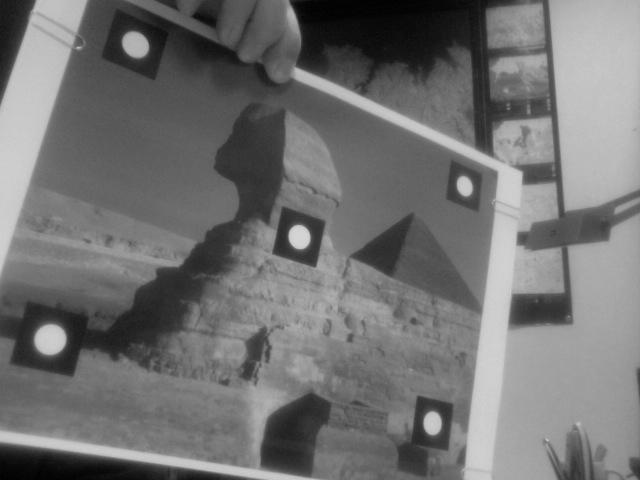
\includegraphics[width=0.48\textwidth]{img/I1.jpg}}
  \hspace{0.030\textwidth}
  \subfloat[Deuxième image]{\label{img2}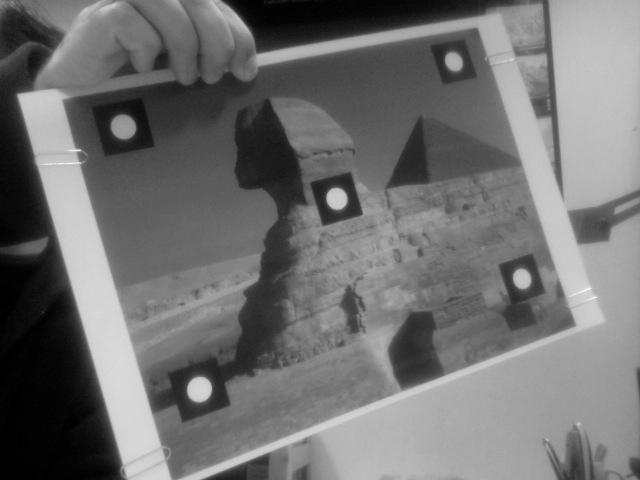
\includegraphics[width=0.48\textwidth]{img/I2.jpg}}
  \caption{Les deux images comportant les points à mettre en correspondance}
  \label{fig_init}
\end{figure}

\subsection{Question 3}
L'estimation semble précise. On peut le vérifier avec la question suivante, pour visualiser l'erreur.

\subsection{Question 4}
On transfère les points $(u2_i, v2_i)$ dans l'image 1 grâce à l'homographie, puis on compare les
résultats avec les vrais points $(u1_i, v1_i)$. On calcule ainsi l'erreur commise et on l'affiche par
un cercle centré sur le point calculé, de rayon dix fois l'erreur commise (fig. \ref{erreur}).

\begin{figure}[!ht]
    \center
    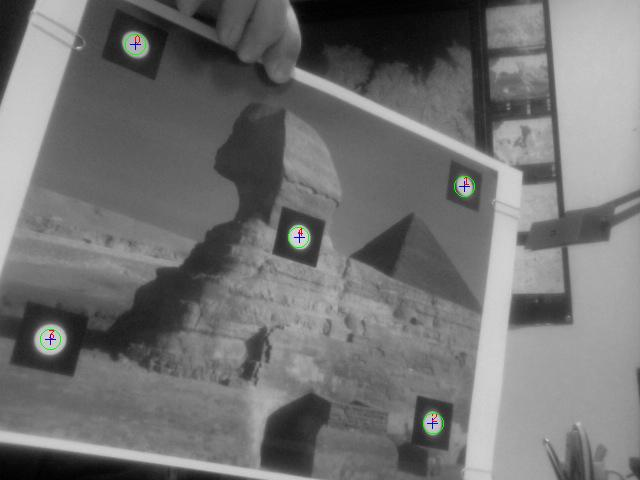
\includegraphics[width=0.68\textwidth]{img/resultat.jpg}
    \caption{Visualisation de l'erreur de calcul induise par l'homographie}
    \label{erreur}
\end{figure}

\subsection{Question 5}
D'après les questions précédentes, on peut maintenant calculer la correspondance des points d'une image à
l'autre. Dans cette question, on transfère tous les points de la deuxième image dans la première en utilisant
cette méthode. Le résultat nous donne notre première mosaïque (fig. \ref{mosaique}). Pour la visualisation,
chacune des deux images à une transparence de 50\%, les zones communes apparaissent donc sans aucune
transparence.

\begin{figure}[!ht]
    \center
    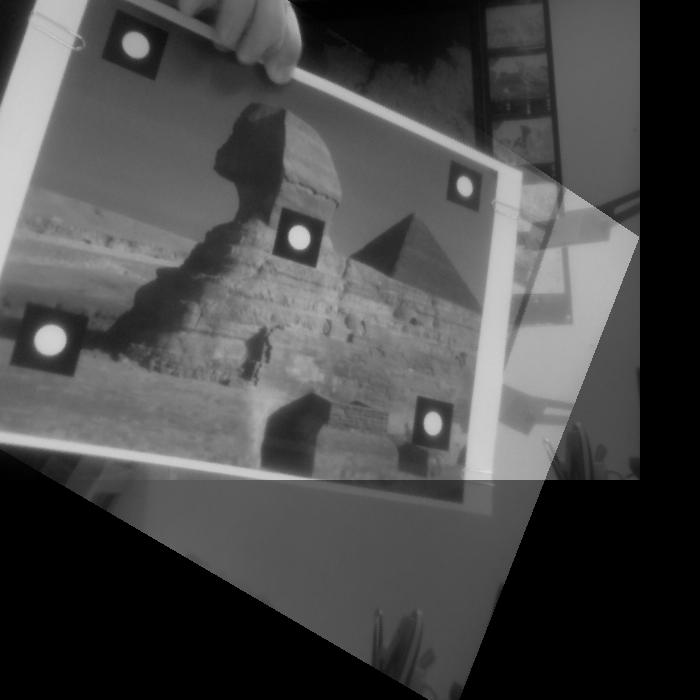
\includegraphics[width=0.68\textwidth]{img/resultat_mosaic.jpg}
    \caption{Mosaïque obtenue par le transfère des points de la deuxième image dans la première.}
    \label{mosaique}
\end{figure}

\section{Random sample consensus}

\subsection{Question 6}
On affiche les mises en correspondances acquises automatiquement (via OpenCV, ou vpBrief, ou autre \ldots),
figure \ref{corres}.

\begin{figure}[!ht]%htp]
  \centering
  \subfloat[Première image]{\label{img1}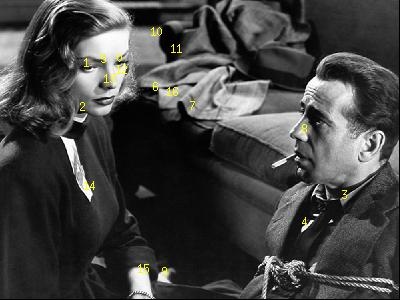
\includegraphics[width=0.48\textwidth]{img/resultat_I1.jpg}}
  \hspace{0.030\textwidth}
  \subfloat[Deuxième image]{\label{img2}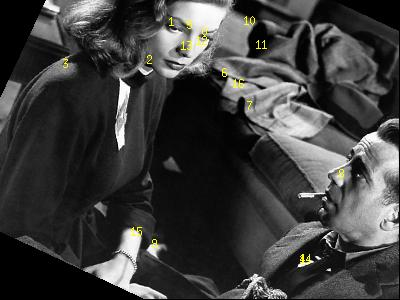
\includegraphics[width=0.48\textwidth]{img/resultat_I2.jpg}}
  \caption{Point mis en correspondance de manière automatique}
  \label{corres}
\end{figure}

On peut constater quelques erreurs de mise en correspondance, pour les visualiser plus rapidement, on peut
tracer des droites entre les correspondances, les outliners apparaissent naturellement à l'oeil (fig.
\ref{corres2}).

\begin{figure}[!ht]
    \center
    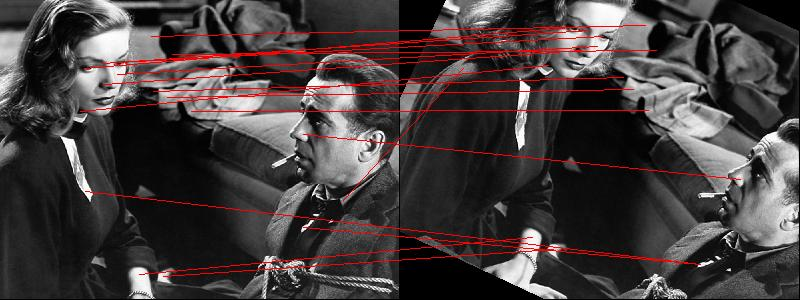
\includegraphics[width=1\textwidth]{img/resultat_I.jpg}
    \caption{Mise en correspondance graphique, les erreurs apparaissent.}
    \label{corres2}
\end{figure}

\subsection{Question 7}
On applique directement l'algorithme développé dans la première partie. Les erreurs ne sont pas raisonnables.
Les quelques erreurs de correspondances suffisent pour fausser le calcul de l'homographie.

\subsection{Question 8}
Pour pallier à ce problème, il faut impérativement détecter les erreurs de matching et les éliminer.
On utiliser un algorithme basé sur RANSAC (pour RANdom SAmple Consensus) permet de détecter rapidement les
outliners des inliner dans notre mise en correspondance. 

Le résultat de notre implémentation de RANSAC est visible figure \ref{ransac}. Les inliners sont tracés en
vert tandis que les outliners sont tracés en rouge.

\begin{figure}[!ht]
    \center
    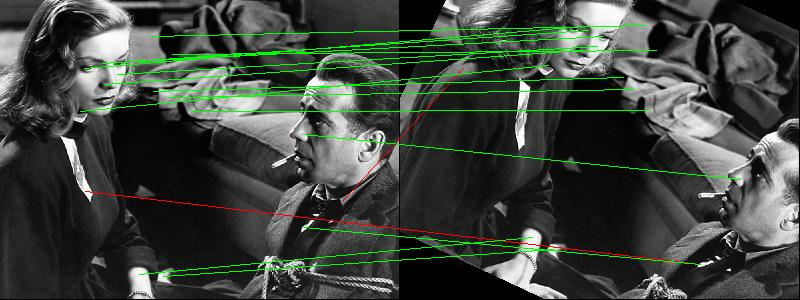
\includegraphics[width=1\textwidth]{img/resultat_ransac.jpg}
    \caption{Mise en évidence des inliners et outliners grâce à RANSAC.}
    \label{ransac}
\end{figure}

\subsection{Question 9}
La contrainte à respecter pour faire une mosaïque avec cette technique est liée à l'homographie. En effet,
l'homographie permet de trouver la transformation d'un plan par rapport à un autre (rotation + translation).
Notre <<image>> à reconstituer doit donc représenter un plan.

\end{document}
%\begin{figure}[!ht]%htp]
%  \centering
%  \subfloat[Image d'origine]{\label{fig:loup}\includegraphics[width=0.48\textwidth]{img/loup.png}}
%  \hspace{0.030\textwidth}
%  \subfloat[Gradient de l'image]{\label{fig:gradient}\includegraphics[width=0.48\textwidth]{img/energie.png}}
%  \caption{Loup.pgm et calcul de l'énergie associée}
%  \label{fig:init}
%\end{figure}

%\begin{figure}[!ht]
%    \center
%    \includegraphics[width=0.48\textwidth]{img/seams.png}
%    \caption{Coutures d'énergie minimales}
%    \label{seams}
%\end{figure}
